\documentclass[a4paper,11pt]{article}
\usepackage[T1]{fontenc}      % codifica dei font
\usepackage[utf8]{inputenc}
\usepackage[italian]{babel}
\usepackage{lipsum}
\usepackage{comment}
\usepackage{url}
\usepackage{amsfonts}
\usepackage{graphicx}
\begin{document}
% lettere accentate da tastiera
% lingua del documento
% genera testo fittizio
% per scrivere gli indirizzi Internet
\author{Linpeng Zhang}
\title{Tutorato AFL}
\maketitle
\begin{abstract}
    Per errori/dubbi/problemi: linpeng.zhang@studenti.unipd.it.
\end{abstract}
\tableofcontents
\section{Lez10}
\subsection{Esercizi}
\begin{enumerate}
    \item  Il seguente linguaggio è regolare? $L =\{ a^k b^k c^i | i\leq k\}$;
    \item  Il seguente linguaggio è context free? $L =\{ a^k b^k c^i | i\leq k\}$;
    \item  Il seguente linguaggio è regolare? $L =\{$ stringhe con un numero pari di a $\}$;
    \item  Il seguente linguaggio è context free? $L =\{$ stringhe con un numero pari di a $\}$;
\end{enumerate}
\subsection{Soluzioni}
\begin{enumerate}
    \item no, dimostrare con il PL per i linguaggi regolari;
    \item no. Una traccia della dimostrazione è la seguente:\\
    Sia (per assurdo) L un linguaggio CFL. Sia $n$ la lunghezza data dal PL. Prendiamo una stringa $z$ tale che $|z| \geq n$.
    Sia $z=a^nb^nc^n= uvwxyz, \ |vwx| \leq n, vx \neq \epsilon$.\\
    Come è fatto $vx$? Da al più due caratteri contigui tra (a, b, c).
    Se è fatto da soli $a$, allora $z=uv^0wx^0y=$ chiaramente $\#a\neq \#b$.
    Se è fatto da soli $b$, allora $z=uv^0wx^0y=$ chiaramente $\#a\neq \#b$.
    Se è fatto da soli $c$, allora $z=uv^2wx^2y=$ chiaramente $\#c > \#a$ (oppure b).
    Se $vx$ è composto da a e b, allora $z=uv^0wx^0y=$ chiaramente $\#c > \#a$ (oppure b).
    Se $vx$ è composto da b e c, allora $z=uv^2wx^2y=$ chiaramente $\#c > \#a$.
    \item sì. Una regexp è $R=(aa)^{*}$;
    \item sì: un linguaggio regolare è context free;
\end{enumerate}
\subsection{Traccia alle risposte delle domande della simulazione}
\begin{enumerate}
    \item si dimostra per induzione sul numero di derivazioni; con una derivazione si deriva $\epsilon$ che banalmente soddisfa la proprietà; con $n+1$ derivazioni, dopo la prima si ha $aS$ oppure $aSbS$ e con altre n derivazioni si ha $aw'$ oppure $aw'bw''$ con $w', w''$ che soddisfano la proprietà. Naturalmente anche $aw'$ la soddisfa (visto che si aggiunge una a all'inizio) e lo stesso per $aw'bw''$, visto che si aggiunge una a all'inizio e una b che è matchata dalla a aggiunta all'inizio;
    \item \begin{minipage}{\linewidth}
        $\delta (q, \epsilon, S) = \{(q,aS), (q,aSbS), (q, \epsilon)\}$\\
        $\delta (q, a, a) = \{(q,\epsilon)\}$\\
        $\delta (q, b, b) = \{(q,\epsilon)\}$\\
    \end{minipage}
    \item un DPDA che accetta per stati finiti riconosce tutti i linguaggi regolari (basta ignorare lo stack), ma non tutti i CFL: ad esempio $ww^r$ no e un esempio è data dalle stringhe $0110$ e $01100110$. L'automa deterministico dopo aver letto la prima stringa (che dovrebbe accettare) deve aver consumato lo stack (prima mette 01 in pila poi leggendo 10 matcha lo stack). Ma allora se leggesse 01100110 come si dovrebbe comportare? Avrebbe già svuotato lo stack consumando solo metà input!\\
    Un DPDA che accetta per stack vuoto accetta solo linguaggi accettati da DPDA che hanno la proprietà del prefisso. L'intuizione è simile: se il DPDA legge x, deve averlo consumato. Quindi non può leggere x seguito da qualcos'altro, ovvero deve esserci sempre la proprietà del prefisso.\\
    Importanza: si è dimostrato che se un DPDA riconosce un linguaggio, allora tale linguaggio non è inerentemente ambiguo.
    \item è chiaro che l'automa non svuoti mai la pila, quindi si presume che riconosca per stato finale. Quando legge una a la mette in cima. Quando legge una b, se c'è una a in cima la toglie, altrimenti si blocca (non ha transizioni). Quindi si può intuire che l'automa riconosca l'insieme delle stringhe per cui ogni prefisso ha un numero di a maggiore o uguale al numero di b. Usare la costruzione vista a lezione per la conversione.
    \item (a): il consiglio presente nella consegna vi dice già come risolvere l'esercizio. Caso base: 1 derivazione, si deriva la stringa $\epsilon$ che è banalmente bilanciata. Con n+1 derivazioni, la prima può usare una delle due produzioni. Seguono n derivazioni, che portano ad avere o la concatenazione di due stringhe bilanciate o del tipo $(w)$ con w bilanciato. Naturalmente in entrambi i casi la proprietà è rispettata e si ha la tesi.
    \\(b): non genera ad esempio $()()$.
    \item \begin{minipage}{\linewidth}
        $[qXq] \rightarrow a[qYq][qZq]$\\
        $[qXq] \rightarrow a[qYp][pZq]$\\
        $[qXp] \rightarrow a[qYq][qZp]$\\
        $[qXp] \rightarrow a[qYp][pZp]$\\
    \end{minipage}
    \item non fatto;
    \item non fatto;
    \item se una grammatica ha h simboli, allora una parola w lunga almeno $2^h$ richiederà che due simboli si ripetano nell'albero di derivazione. Sia A il simbolo che si ripete, allora l'albero radicato in A deriva o xAy o w. Chiaramente si può ripetere "xAy" infinite volte. Si ha quindi il PL.
      %   \item si può dimostrare che A genera $L_A=\{a^nb^m|n=m+1$ oppure $n=m$ con $n>0,m\geq 0\}$, B genera $L_B=\{a^nb^m|m=n+1$ oppure $n=m$ con $m>0,n\geq 0\}$. Dalle due asserzioni precedenti si dimostra che S genera $L_S=\{a^nb^m|n=m+1$ oppure $n=m$ con $n,m>0\}$: infatti S produce le stringhe che produce B con una a all'inizio, e la correttezza segue dalla definizione.\\
   %  Un automa a pila che accetta tale linguaggio è:\\
  %  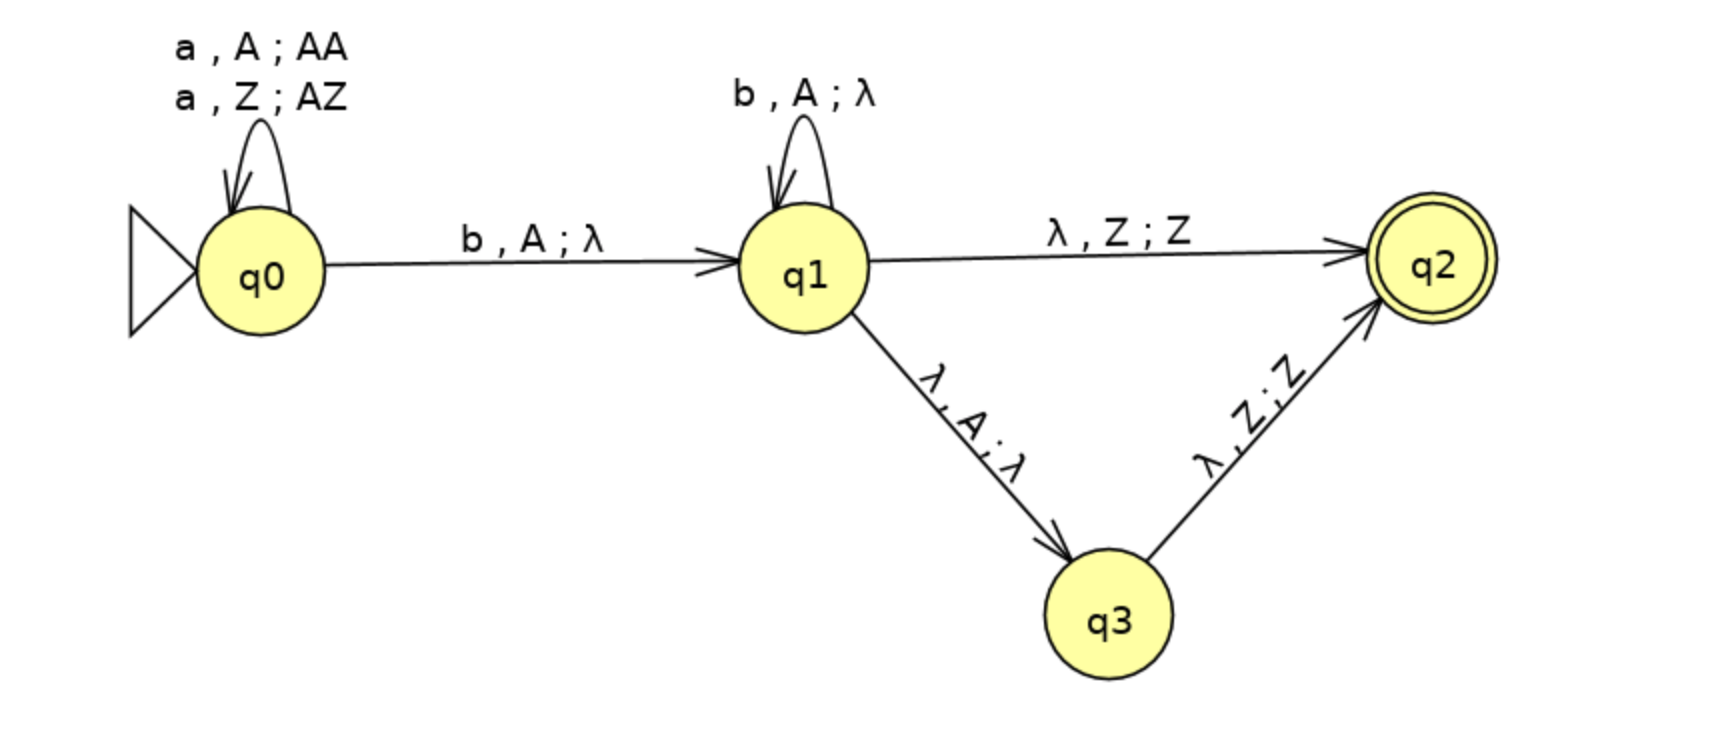
\includegraphics[scale=0.5]{Lez7sol6.png}
\end{enumerate}

\begin{comment}
          \item \begin{minipage}{\linewidth}
        $S \rightarrow [qZq]$\\
        $(1) [qZq] \rightarrow 1[q1q][qZq]$\\
        $(2) [qZq] \rightarrow 0[q0q][qZq]$\\
        $(3) [q1q] \rightarrow 0$\\
        $(4) [q0q] \rightarrow 1$\\
        $(5) [q1q] \rightarrow 1[q1q][q1q]$\\
        $(6) [q0q] \rightarrow 0[q0q][q0q]$\\
        $(7) [qZq] \rightarrow \epsilon$\\
      \end{minipage}
       \item Sia data la CFG:\\
     \begin{minipage}{\linewidth}
        \centering $S \rightarrow aB$\\
        \centering $B \rightarrow Ab\ |\ b$\\
        \centering $A \rightarrow aB\ |\ a$\\
    \end{minipage}
    \\Dire: linguaggio accettato e definire un automa che accetti tale linguaggio.
\end{comment}
    % Bibliografia
    %\begin{thebibliography}{9}
        %  Alcune soluzio
    %\end{thebibliography}
    \end{document}